\section{Reporte de funcionalidades}
\subsection{Funcionalidades especificadas}
\begin{itemize}
    \item \textbf{RF1 - Gestionar la información básica.} \\
    \textit{Permite la gestión apropiada de la información de la mascota, como es:
    su nombre, peso, altura, posibles comentarios y la imagen.}
    \item \textbf{RF2 - Registrar en calendarios los paseos.} \\
    \textit{Calendario que permite registrar el día y hora de un paseo para una mascota, ingresando el responsable de dicha tarea.}
    \item \textbf{RF3 - Calendario de alimentación de la mascota.} \\
    \textit{Brinda la posibilidad de registrar en el calendario el responsable de alimentar una mascota para un día y hora en especifico.}
    \item \textbf{RF4 - Registro de actividad realizada.} \\
    \textit{Permite registrar una activad ya realizada, la misma puede ser un paseo, alimentación u otra, indicando un nombre, usuario, perro y recorrido o alimento según su tipo.}
    \item \textbf{RF5 - Agendar servicio veterinaria.} \\
    \textit{Funcionalidad que habilita el registar un servicio de cuidado en una veterinaria, como puede ser corte de pelos, uñas, etc.}
    \item \textbf{RF6 - Recordatorios vía email.} \\
    \textit{Envía recordatorio vía correo electrónico y notificaciones de sistema a los responsables de las actividades agendadas previamente.}
\end{itemize}

\subsection{Funcionalidades no especificadas}
\begin{itemize}
    \item \textbf{RF6 - Recordatorios vía email.} \\
    \textit{Carga una colección de datos al sistema para poder operar o probar el resto de su funcionamiento.}
    \item \textbf{RF8 - Agregar usuario.} \\
    \textit{Permite registrar un usuario ingresando nombre y mail, dichos usuarios serán utilizados para la asignación de tareas.}
\end{itemize}




\section{Inventarios de pruebas}

\subsection{Técnicas}
Para la siguiente revisión de cobertura de pruebas, se utilizó el componente incorporado en entorno de desarrollo "IntelliJ IDEA", de esta manera poder obtener la totalidad de lineas de códigos que son comprendidas por las pruebas, mientras que para la verificación de pruebas de caja negra, se tomara como valida únicamente una prueba, siempre y cuando contenga los siguientes elementos:
\begin{itemize}
    \item E1 - Identificador de requerimiento funcional que se prueba
    \item E2 - Requisitos previos.
    \item E3 - Datos de entradas correctos e incorrectos.
    \item E4 - Salida de la prueba esperada.
    \item E5 - Salida de la prueba obtenida.
\end{itemize}

Ponderamos cada uno de estos elementos de igual manera para indicar que una prueba 100\% completa tiene los 5 elementos.

\subsection{Revisión}
Pruebas caja negra:
\prettyTable{|p{4cm}|l|l|l|l|l|l|}{
    \textbf{Requerimiento funcional} & \textbf{E1} & \textbf{E2}  & \textbf{E3}  & \textbf{E4}  & \textbf{E5} & \textbf{Cobertura} \\ \hline
    \textbf{RF1} & \xmark & \xmark & \cmark & \cmark & \xmark & 40\% \\ \hline
    \textbf{RF2} & \xmark & \cmark & \cmark & \cmark & \xmark & 60\% \\ \hline
    \textbf{RF3} & \xmark & \cmark & \cmark & \cmark & \xmark & 60\% \\ \hline
    \textbf{RF4} & \xmark & \cmark & \cmark & \cmark & \xmark & 60\% \\ \hline
    \textbf{RF5} & \xmark & \cmark & \cmark & \cmark & \xmark & 60\% \\ \hline
    \textbf{RF6} & \xmark & \xmark & \cmark  & \xmark & \xmark & 60\% \\ \hline
    \textbf{RF7} & \xmark & \xmark & \xmark & \xmark & \xmark & 0\% \\ \hline
    \textbf{RF8} & \xmark & \xmark & \xmark & \xmark & \xmark & 0\% \\ \hline
}

Pruebas caja blanca:
\begin{figure}[H]
    \centering
    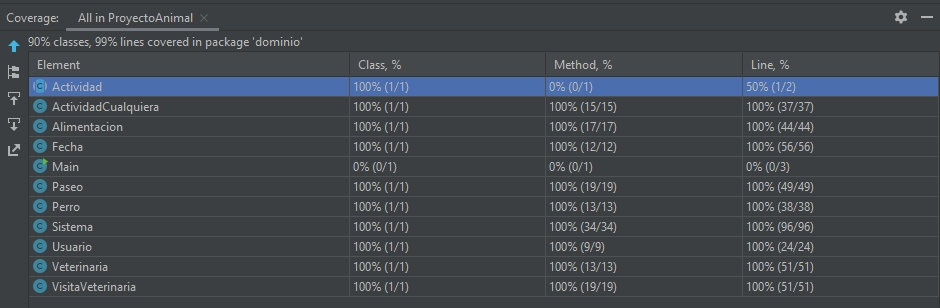
\includegraphics[scale =1.8]{Files/coverturaUnitTests.jpg}
    \caption{Evidencia cobertura de pruebas unitarias}
    \label{fig:clases}
\end{figure}

Resumen:
\prettyTable{|p{4cm}|p{4cm}|p{4cm}|}{
    \textbf{Requerimiento funcional} & \textbf{Cobertura de las pruebas de caja negra} & \textbf{Cobertura de las pruebas de caja blanca} \\ \hline
    \textbf{RF1} & 100\% &  40\% \\ \hline
    \textbf{RF2} & 100\% & 60\%  \\ \hline
    \textbf{RF3} & 100\% & 60\%  \\ \hline
    \textbf{RF4} & 100\% & 60\%   \\ \hline
    \textbf{RF5} & 100\% & 60\%  \\ \hline
    \textbf{RF6} & 100\% &  60\%  \\ \hline
    \textbf{RF7} & 100\% & 0\%  \\ \hline
    \textbf{RF8} & 100\% & 0\%  \\ \hline
}

